\documentclass{article}
\usepackage{graphicx}
\graphicspath{ {./images/} }
\usepackage{parskip}

\renewcommand{\figurename}{Abb.}

\begin{document}

\begin{titlepage}
    \centering
NVS- Projekt 2020/21, 5AHIF

\vskip4cm
    {\bfseries\Large
        \huge\underline{MLT3- Simulator}

	Maurice Putz\\
    }
    
\includegraphics[width=6cm]{mlt3logo.png} % also works with logo.pdf
    \vskip6cm
 8. Jänner 2021\\
\end{titlepage}

\pagenumbering{gobble}
\newpage
\tableofcontents
\newpage
\pagenumbering{arabic}

\section{Beschreibung}

Der MLT-3 Simulator dient einer Simulierung der Leitungskodierung MLT-3. Vom Sender werde zuerst ASCII-Zeichen 
ins Dezimal System ungewandelt, dann weiter in binären Code und dann mittels der MLT-3 Signalform welche aus
den binären teilen besteht, übertragen. Die MLT-3 codierte Datenfolge wird nun beim Empfänger zurück ins binäre System
übersetzt, danach ins dezimale und schlussendlich wieder als ACII-Zeichen dekodiert ausgegeben.

Das Programm gibt diesen Vorgang standardgemäß auf der Konsole als Tabelle formatiert aus. Es exisiteren weitere
Optionen und Funktionen, welche in Abschnitt "Funktionen und Optionen", genauer beschrieben sind.

\subsection{MLT-3 Zusammenfassung}

MLT steht für Multilevel Transmission Encoding, die drei am Ende steht für "3 levels", also die drei Spannungsformen welche eine
MLT-3 kodierte Datenfolge haben kann. Diese drei Spannungen, was die Folge zu einem Ternären Signal macht,
werden in einer Folge meisten als +, 0 und - Dargestellt, wie man gut in Abb. 1 erkennen kann.

MLT-3 ändert den Datenstrom bei jeder logischen Eins, bei einer logischen Null ändert sich der Zustand der Leitung nicht und das
gleiche Zeichen wird einfach ein weiteres Mal übernommen. Die bringt vor allem der Vorteil, dass die Kodierung viel weniger Bandbreite als
andere wie zum Beispiel NRZ (No Return to Zero) benötigt, da eben nur bei einer Änderung mit einer logischen Eins, die Spannung geändert wird.

\begin{center}
\begin{figure}[h]
    \centering
    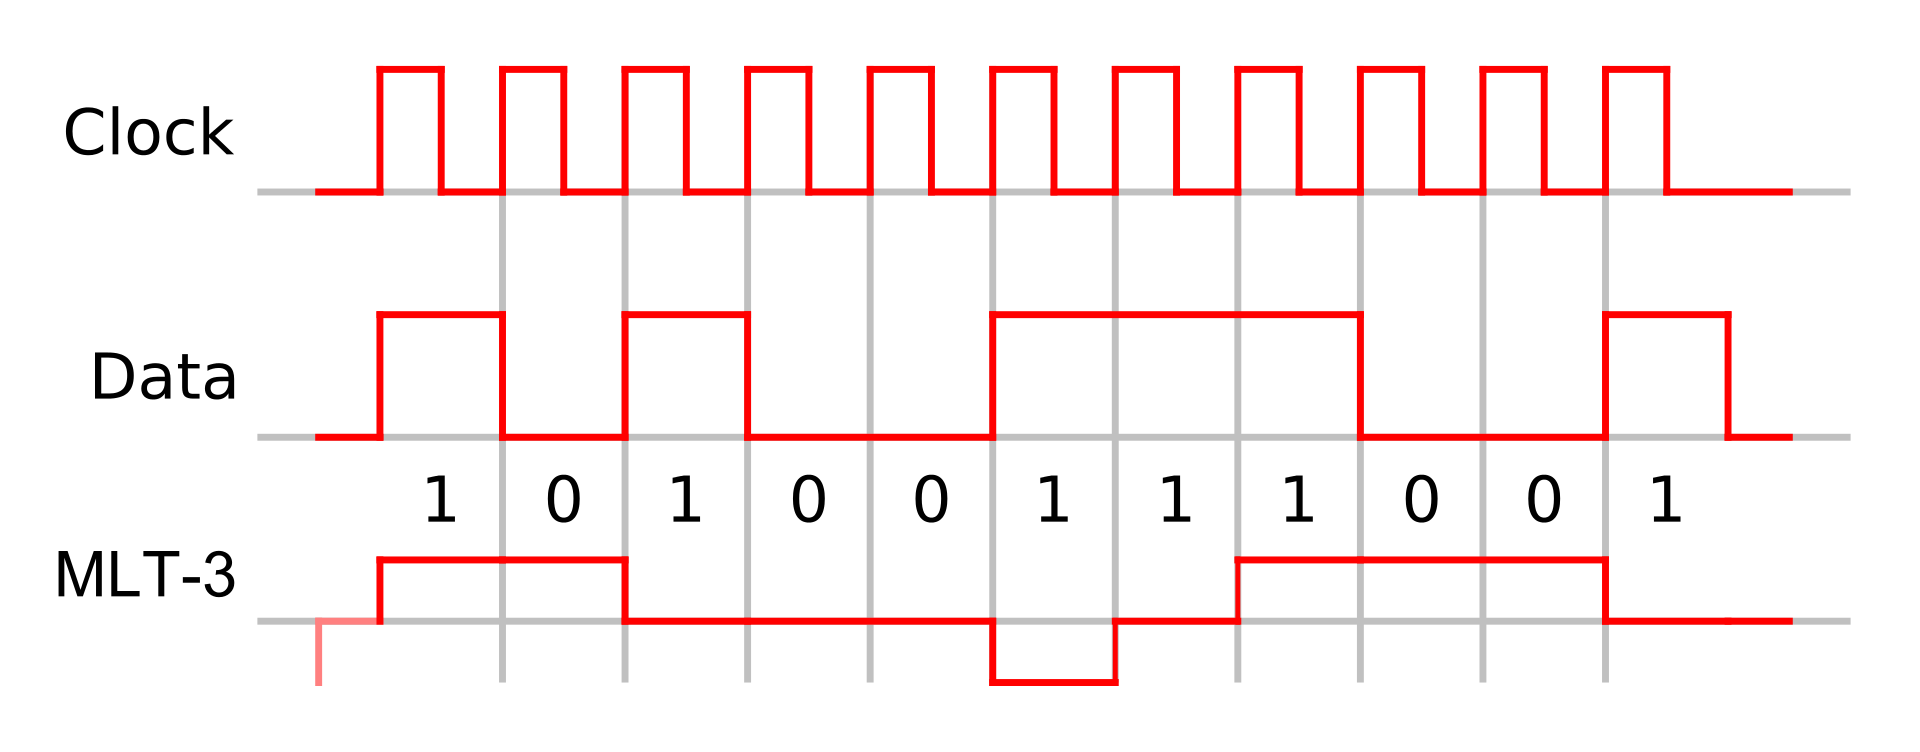
\includegraphics[width=\textwidth]{MLT3encoding.png}
    \caption{Clock dient zur Markierung der Übergangszeitpunkte}
\end{figure}
\end{center}
\break

Die Spannung ändert sich wie bereits erwähnt jedes Mal wenn eine logische Eins verabreitet wird. Diese Änderung variert folgender
Reihenfolge:

\begin{enumerate}
	\item Von 0 auf +
	\item Von + auf 0
	\item Von 0 auf -
	\item Von - auf 0
\end{enumerate}

Diese vier Schritte wiederholen sich jedes Mal bei einer logischen Eins in genau dieser Reihenfolge.

\section{Funktionen und Optionen}

\begin{center}
\begin{figure}[h]
    \centering
    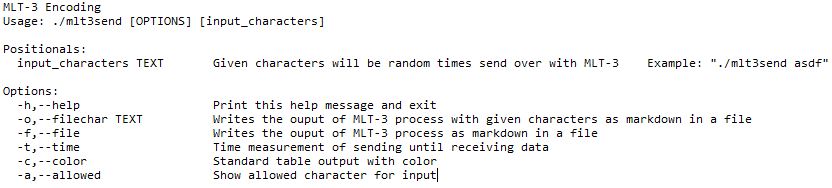
\includegraphics[width=16cm]{climenu.png}
    \caption{Hilfe des Programms in der Kommandozeile}
\end{figure}
\end{center}

Option \textbf{-h,--help}:\\
Zeigt die Hilfe für das Programm an, liefert das Menü wie in Abb. 2 zurück.
\begin{itemize}
	\item \underline{Eingabe:} ./mlt3send -h
	\item \underline{Ausgabe:} [Siehe Abb. 2]\\
\end{itemize}

Option \textbf{-o,--filechar TEXT}:\\
Startet das Programm und schreibt das Ergebnis als markdown in eine Datei, Speicherort der Datei wird nach Aufruf auf der Konsole ausgegeben.
Erwartet ASCII kodierbare Character als eingabe.
Beispiel: 
\begin{itemize}
	\item \underline{Eingabe:} ./mlt3send -o asdf
	\item \underline{Ausgabe:}

[NOTE]\\
The result is saved to the location: /home/maurice/Desktop/mlt3.mkd\\
It is formated as markdown.\\
\end{itemize}

Flag \textbf{-f,--file}:\\
Startet das Programm mit zufällig gewählten ASCII-Zeichen und schreibt sie als mardown in eine Datei, Speicherort der Datei wird nach Aufruf auf der Konsole ausgegeben.
Beispiel: 
\begin{itemize}
	\item \underline{Eingabe:} ./mlt3send -f
	\item \underline{Ausgabe:}

[NOTE]\\
The result is saved to the location: /home/maurice/Desktop/mlt3.mkd\\
It is formated as markdown.\\
\end{itemize}

Flag \textbf{-t,--time}:\\
Startet das Programm und gibt das Ergebnis auf der Konsole aus. Zusätzlich wird am Ende die gemessene Zeit in Nano und Mikrosekunden ausgegeben. Der Grund für die beiden
Einheiten ist, dass manchmal, wenn zufällig und ein Zeichen übertragen wird, oder der Computer sehr schnell ist, auf dem das Programm ausgeführt wird, dies unter
einer Mikrosekunde passiert.

Die gemessene Zeit wird mit Start des Sende-Threads angefangen, und endet mit der Verarbeitung aller Daten durch den Empfängerthread. Die Ausgabe in die Konsole oder
das schreibeun in eine Datei wird \underline{nicht} mitgemessen.

Flag \textbf{-c,--color}:\\
Startet das Programm mit zufällig gewählten ASCII-Zeichen

Flag \textbf{-a,--allowed}:\\
Nope



\section{Quellen}

\begin{itemize}
	\item https://de.wikipedia.org/wiki/MLT-3-Code
	\item https://de.wikipedia.org/wiki/Tern%C3%A4res_Signal
	\item Folie 21. "Encoding and Decoding" aus dem NVS Unterricht
\end{itemize}

\textbf{Alle benutzen Bilder sind frei für akademische Zwecke zu benutzen oder das Urheberrecht liegt beim Verfasser (Maurice Putz)}

\end{document}